\documentclass{amsart}

\usepackage{tikz}
\pgfrealjobname{tikz-figures}

\begin{document}

\begin{figure}
\centering
\beginpgfgraphicnamed{figure1}%
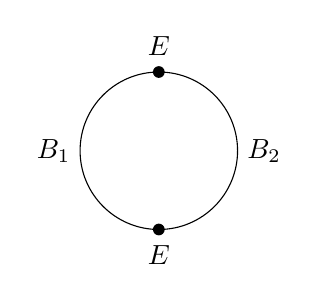
\begin{tikzpicture}[%every label/.style={green}
]
\node[fill=black, circle, label=below:$E$, inner sep=1.5pt](S) at (0,0) {};
\node[fill=black, circle, label=above:$E$, inner sep=1.5pt](N) at (0,2) {};
\draw (S) arc  (-90:90:1);
\draw (N) arc  (90:270:1);
\node[left] at (-1,1) {$B_1$};
\node[right] at (1,1) {$B_2$};
\end{tikzpicture}
\endpgfgraphicnamed%
\mbox{} % <-- weird, doesn't compile unless I put something here after the \endpgfgraphicnamed...? -S
\caption{Combining two balls to get a full boundary.}\label{blah3}\end{figure}

\begin{figure}
\centering
\beginpgfgraphicnamed{figure2}%
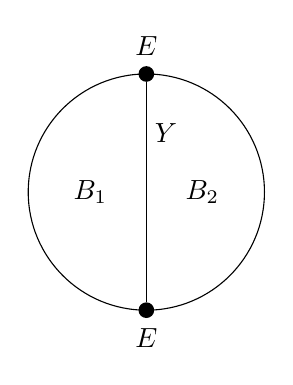
\begin{tikzpicture}[%every label/.style={green},
				x=1.5cm,y=1.5cm]
\node[fill=black, circle, label=below:$E$, inner sep=2pt](S) at (0,0) {};
\node[fill=black, circle, label=above:$E$, inner sep=2pt](N) at (0,2) {};
\draw (S) arc  (-90:90:1);
\draw (N) arc  (90:270:1);
\draw (N) -- (S);
\node[left] at (-1/4,1) {$B_1$};
\node[right] at (1/4,1) {$B_2$};
\node at (1/6,3/2)  {$Y$};
\end{tikzpicture}
\endpgfgraphicnamed%
\mbox{} % <-- weird, doesn't compile unless I put something here after the \endpgfgraphicnamed...? -S
\caption{From two balls to one ball.}\label{blah5}\end{figure}


\end{document}

